\documentclass{article}
\usepackage[paperwidth=12.5cm,paperheight=5.85cm,margin=0pt,
            noheadfoot,nomarginpar]{geometry}
\usepackage{amsmath,amssymb}
\usepackage{tikz}
\pagestyle{empty}
\setlength{\parindent}{0pt}
\setlength{\topskip}{0pt}
\setlength{\abovedisplayskip}{0pt}

\begin{document}
\noindent\centering\vspace*{-0.1cm}
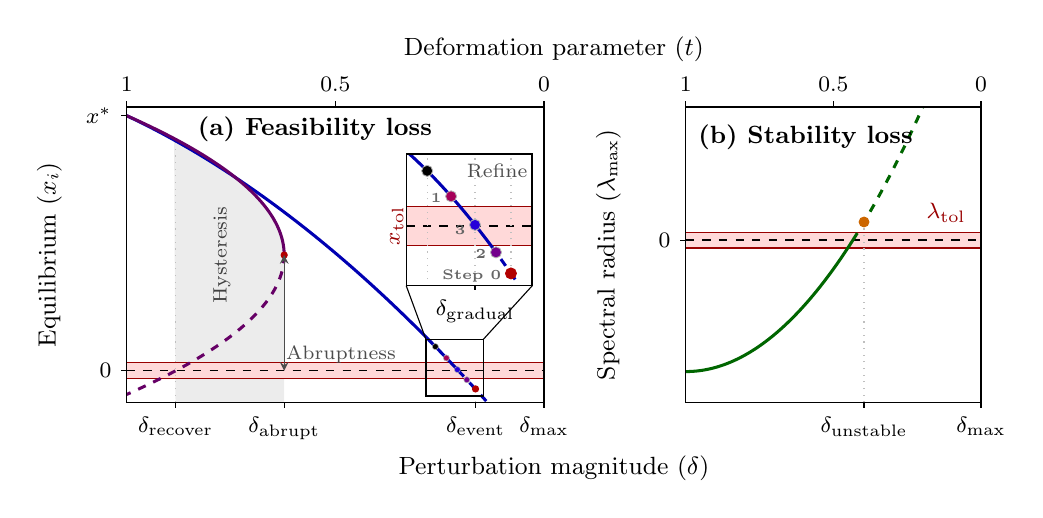
\begin{tikzpicture}[
  >=stealth,
  stable/.style  ={line width=1.1pt, blue!70!black},
  unstable/.style={line width=1.1pt, blue!70!black, dashed},
  stable2/.style  ={line width=1.1pt, violet!80!black},
  unstable2/.style={line width=1.1pt, violet!80!black, dashed},
  stableG/.style  ={line width=1.1pt, green!40!black},
  unstableG/.style={line width=1.1pt, green!40!black, dashed},
  thres/.style={red!60!black, dashed, line width=0.6pt},
  vguide/.style={gray!50, dotted, thin},
  reddot/.style={fill=red!70!black, draw=red!70!black, circle,
                 inner sep=0pt, minimum size=2.2pt},
  orangedot/.style={fill=orange!80!black, draw=orange!80!black, circle,
                    inner sep=0pt, minimum size=3.5pt},
  bisecdot/.style={circle, inner sep=0pt, minimum size=4pt,
                   draw=black!30, line width=0.3pt},
  itlabel/.style ={font=\tiny\bfseries, black!60},
  boxframe/.style={black, line width=0.5pt},
  insetframe/.style={draw=black!70, line width=0.4pt, fill=white, fill opacity=0.94,
                     rounded corners=1.2pt},
]

% Panel dimensions
\def\dmax{5.3}
\def\W{5.3}
\def\H{3.75}
\def\gap{1.8}

\def\xtol{0.23}
% Visual half-width of the tolerance band (thinner than xtol)
\def\bandw{0.10}
% Vertical shift so that x_i=0 is above the frame bottom,
% leaving room for negative values below
\def\yshift{0.4}

% =====================================================
% PANEL (a): Feasibility loss
% =====================================================
% Blue curve: f(d) = 3.24 - 0.471*d - 0.0707*d^2
%   Zero crossing at d=4.21; crossing -xtol=-0.23 at d=4.43
\def\dcAzero{4.21}
\def\dcA{4.43}

% Fold: x*=3.24, tfold=1.47, dfold=2.0
%   afold = 2.0/(3.24-1.47)^2 = 0.6384
%   x_i=0 at delta=0.62;  stable branch at delta_recover: x_i=2.95
\def\tfold{1.47}
\def\dfold{2.0}
\def\afold{0.6384}
\def\drecover{0.62}
\def\xrecover{2.95}

\begin{scope}[shift={(0,0)}]
  \begin{scope}
    \clip (0,0) rectangle (\W, \H);

    % Hysteresis shading: under stable branch
    \fill[gray!15]
      (\drecover, 0) --
      plot[smooth,variable=\t,domain=\xrecover:\tfold,samples=30]
        ({\dfold - \afold*(\t-\tfold)*(\t-\tfold)}, {\t + \yshift}) --
      (\dfold, 0) -- cycle;

    % Tolerance band around 0 (light red, thin)
    \fill[red!15] (0, {\yshift - \bandw}) rectangle (\W, {\yshift + \bandw});
    % Grey zero line (on top of band)
    \draw[black, dashed, line width=0.5pt] (0,\yshift) -- (\W,\yshift);
    % Red border lines on band edges
    \draw[red!60!black, line width=0.4pt] (0,{\yshift - \bandw}) -- (\W,{\yshift - \bandw});
    \draw[red!60!black, line width=0.4pt] (0,{\yshift + \bandw}) -- (\W,{\yshift + \bandw});

    % Vertical guide lines
    \draw[vguide] (\dcA,0) -- (\dcA,{\yshift - \xtol});
    \draw[vguide] (\drecover,0) -- (\drecover,{\xrecover + \yshift});

    % Curve 1: smooth decreasing — solid until zero, dashed beyond
    \draw[stable] plot[smooth,domain=0:\dcAzero,samples=60]
      (\x, {3.24 - 0.471*\x - 0.0707*\x*\x + \yshift});
    \draw[unstable] plot[smooth,domain=\dcAzero:\dmax,samples=30]
      (\x, {3.24 - 0.471*\x - 0.0707*\x*\x + \yshift});
    % Bisection iteration dots on main curve, mapped inside the zoom rectangle
    % Zoom rect x=[3.8,4.53], mapping: main_x = 3.8 + inset_x*(0.73/4.2)
    %   inset 0.7 -> 3.92,  inset 1.5 -> 4.06,  inset 3.0 -> 4.32,  inset 2.3 -> 4.20
    \node[circle, inner sep=0pt, minimum size=2.2pt, fill=black, draw=black!30, line width=0.2pt]
      at (3.92, {3.24 - 0.471*3.92 - 0.0707*3.92*3.92 + \yshift}) {};
    \node[circle, inner sep=0pt, minimum size=2.2pt, fill=blue!35!red, draw=black!30, line width=0.2pt]
      at (4.06, {3.24 - 0.471*4.06 - 0.0707*4.06*4.06 + \yshift}) {};
    \node[circle, inner sep=0pt, minimum size=2.2pt, fill=blue!55!red, draw=black!30, line width=0.2pt]
      at (4.32, {3.24 - 0.471*4.32 - 0.0707*4.32*4.32 + \yshift}) {};
    \node[circle, inner sep=0pt, minimum size=2.2pt, fill=blue!85!red, draw=black!30, line width=0.2pt]
      at (4.20, {3.24 - 0.471*4.20 - 0.0707*4.20*4.20 + \yshift}) {};
    \node[reddot] at (\dcA, {\yshift - \xtol}) {};

    % Curve 2: fold (backward C)
    \draw[stable2] plot[smooth,variable=\t,domain=3.24:\tfold,samples=40]
      ({\dfold - \afold*(\t-\tfold)*(\t-\tfold)}, {\t + \yshift});
    % Unstable branch extended to touch the plot boundary
    \draw[unstable2] plot[smooth,variable=\t,domain=\tfold:-0.5,samples=40]
      ({\dfold - \afold*(\t-\tfold)*(\t-\tfold)}, {\t + \yshift});
    \node[reddot] at (\dfold, {\tfold + \yshift}) {};

    % Abruptness annotation — arrow from x_i=0 up to fold point
    \draw[<->, thin, black!70] (\dfold, \yshift) -- (\dfold, {\tfold + \yshift});
    \node[right, font=\scriptsize, black!70] at (\dfold-0.1, {\yshift + 0.2})
      {Abruptness};

    % Hysteresis label
    \node[font=\scriptsize, gray!50!black, rotate=90] at
      ({(\drecover+\dfold)/2 - 0.1}, {\tfold + \yshift}) {Hysteresis};

    \def\insetx{3.55}
    \def\insety{1.48}

    \draw[-, thin] (3.8,0.8) -- (\insetx,\insety);
    \draw[-, thin] (4.53,0.8) -- (\insetx+1.6,1.48);
    \draw[boxframe] (3.8,0.8) rectangle (4.53,0.08);
    % -----------------------------------------------------
    % Inset: refinement schematic (embedded from refinement_schematic.tex)
    % -----------------------------------------------------
    \begin{scope}[shift={(\insetx,\insety)}, scale=0.38]
      % inset panel background

      \def\iW{4.2}
      \def\iH{4.4}
      \def\iyshift{2}
      \def\ibandw{0.65}
      \def\dzero{2.835}
      \def\dprev{0.7}
      \def\devent{3.5}
      \def\dc{2.3}
      \def\ixshift{2.5}


      \begin{scope}
        \clip (0,0) rectangle (\iW, \iH);

        \fill[red!15] (0,{\iyshift-\ibandw}) rectangle (\iW,{\iyshift+\ibandw});
        \draw[black, dashed, line width=0.5pt] (0,\iyshift) -- (\iW,\iyshift);
        \draw[red!60!black, line width=0.4pt]
          (0,{\iyshift-\ibandw}) -- (\iW,{\iyshift-\ibandw});
        \draw[red!60!black, line width=0.4pt]
          (0,{\iyshift+\ibandw}) -- (\iW,{\iyshift+\ibandw});

        \draw[stable] plot[smooth, domain=0:\dzero, samples=60]
          (\x, {\ixshift - 0.888*\x - 0.08*\x*\x + \iyshift});
        \draw[unstable] plot[smooth, domain=\dzero:\iW, samples=25]
          (\x, {\ixshift - 0.888*\x - 0.08*\x*\x + \iyshift});

        \draw[vguide] (\dprev, 0) -- (\dprev, \iH);
        \draw[vguide] (\dc, 0) -- (\dc, \iH);
        \draw[vguide] (\devent, 0) -- (\devent, \iH);

        \node[bisecdot, fill = black]
          at (\dprev, {\ixshift - 0.888*0.7 - 0.08*0.7*0.7 + \iyshift}) {};

        \node[bisecdot, fill=red!70!black, draw=red!70!black]
          (ev) at (\devent, {\ixshift - 0.888*\devent - 0.08*\devent*\devent + \iyshift}) {};
        \node[itlabel, anchor=east] at ([yshift=-8pt]ev.north) {Step 0};

        \node[bisecdot, fill=blue!35!red]
          (s1) at (1.5, {\ixshift - 0.888*1.5 - 0.08*1.5*1.5 + \iyshift}) {};
        \node[itlabel, anchor=east] at ([yshift=-7pt]s1.north) {1};

        \node[bisecdot, fill=blue!55!red]
          (s2) at (3., {\ixshift - 0.888*3. - 0.08*3.*3. + \iyshift}) {};
        \node[itlabel, anchor=east] at ([yshift=-7pt]s2.north) {2};

        \node[bisecdot, fill=blue!85!red]
          (s3) at (\dc, {\ixshift - 0.888*\dc - 0.08*\dc*\dc + \iyshift}) {};
        \node[itlabel, anchor=east] at ([yshift=-11pt]s3.north) {3};
      \end{scope}

      \draw[boxframe] (0,0) rectangle (\iW,\iH);
      % Refine title — top left inside inset
      \node[font=\scriptsize, black!70, anchor=north west] at (1.7, \iH) {Refine};
      % ---------- Bottom axis ticks ----------
      \draw[line width=0.5pt] (\dc, 0) -- (\dc, -0.14)
        node[below, font=\footnotesize] {$\delta_{\mathrm{gradual}}$};
    \end{scope}
  \end{scope}

  % Box frame
  \draw[boxframe] (0,0) rectangle (\W,\H);

  % Bottom axis (ticks only; shared title placed later)
  \draw (\drecover,0) -- (\drecover,-0.07)
    node[below, font=\footnotesize] {$\delta_{\mathrm{recover}}$};
  \draw (\dfold,0) -- (\dfold,-0.07)
    node[below, font=\footnotesize] {$\delta_{\mathrm{abrupt}}$};
  \draw (\dcA,0) -- (\dcA,-0.07)
    node[below, font=\footnotesize] {$\delta_{\mathrm{event}}$};
  \draw (\dmax,0) -- (\dmax,-0.07)
    node[below, font=\footnotesize] {$\delta_{\max}$};

  % Top axis (ticks only; shared title placed later)
  \draw (0, \H) -- (0, \H+0.07)
    node[above, font=\footnotesize] {$1$};
  \draw (\dmax/2, \H) -- (\dmax/2, \H+0.07)
    node[above, font=\footnotesize] {$0.5$};
  \draw (\dmax, \H) -- (\dmax, \H+0.07)
    node[above, font=\footnotesize] {$0$};

  % Left axis
  \node[left, font=\small, rotate=90, anchor=south] at (-0.7, \H/2)
    {Equilibrium ($x_i$)};
  \draw (0, \yshift) -- (-0.07, \yshift) node[left, font=\footnotesize] {$0$};
  \draw (0, {3.24 + \yshift}) -- (-0.07, {3.24 + \yshift}) node[left, font=\footnotesize] {$x^*$};

  % Threshold label — rotated, acting as y-axis label for the inset
  \node[red!60!black, font=\footnotesize, rotate=90] at (3.43, {1.48 + 0.38*2})
    {$x_{\mathrm{tol}}$};

  % Panel label
  \node[anchor=north east, font=\bfseries\small] at (\W-1.3, \H)
    {(a) Feasibility loss};
\end{scope}

% =====================================================
% PANEL (b): Stability loss
% =====================================================
\def\zeroline{2.06}
\def\ltol{2.29}
% Curve: y(d) = 0.39 + 0.1855*d^2
%   Zero crossing (zeroline=2.06) at d=3.0; crossing ltol=2.29 at d=3.2
\def\dcBzero{3.0}
\def\dcB{3.2}

\begin{scope}[shift={(\W+\gap, 0)}, xscale=0.7075]
  \begin{scope}
    \clip (0,0) rectangle (\W, \H);

    % Tolerance band around 0 (light red, thin)
    \fill[red!15] (0, {\zeroline - \bandw}) rectangle (\W, {\zeroline + \bandw});
    % Grey zero line (on top of band)
    \draw[black, dashed, line width=0.5pt] (0,\zeroline) -- (\W,\zeroline);
    % Red border lines on band edges
    \draw[red!60!black, line width=0.4pt] (0,{\zeroline - \bandw}) -- (\W,{\zeroline - \bandw});
    \draw[red!60!black, line width=0.4pt] (0,{\zeroline + \bandw}) -- (\W,{\zeroline + \bandw});

    \draw[vguide] (\dcB,0) -- (\dcB,\ltol);

    % Solid until zeroline crossing, dashed beyond
    \draw[stableG] plot[smooth,domain=0:\dcBzero,samples=60]
      (\x, {0.39 + 0.1855*\x*\x});
    \draw[unstableG] plot[smooth,domain=\dcBzero:\dmax,samples=30]
      (\x, {0.39 + 0.1855*\x*\x});
    \node[orangedot] at (\dcB, \ltol) {};
  \end{scope}

  % Box frame
  \draw[boxframe] (0,0) rectangle (\W,\H);

  % Bottom axis (ticks only)
  \draw (\dcB,0) -- (\dcB,-0.07)
    node[below, font=\footnotesize] {$\delta_{\mathrm{unstable}}$};
  \draw (\dmax,0) -- (\dmax,-0.07)
    node[below, font=\footnotesize] {$\delta_{\max}$};

  % Top axis (ticks only)
  \draw (0, \H) -- (0, \H+0.07)
    node[above, font=\footnotesize] {$1$};
  \draw (\dmax/2, \H) -- (\dmax/2, \H+0.07)
    node[above, font=\footnotesize] {$0.5$};
  \draw (\dmax, \H) -- (\dmax, \H+0.07)
    node[above, font=\footnotesize] {$0$};

  % Left axis
  \node[left, font=\small, rotate=90, anchor=south] at (-0.99, \H/2)
    {Spectral radius ($\lambda_{\max}$)};
  \draw (0, \zeroline) -- (-0.099, \zeroline)
    node[left, font=\footnotesize] {$0$};

  % Threshold label — inside plot, above band, right-aligned
  \node[red!60!black, font=\footnotesize, anchor=south east] at (\W-0.1, {\zeroline + \bandw})
    {$\lambda_{\mathrm{tol}}$};

  % Panel label
  \node[anchor=north west, font=\bfseries\small] at (0.05, \H-0.1)
    {(b) Stability loss};
\end{scope}

% =====================================================
% Shared axis titles (centered between both panels)
% =====================================================
% Midpoint of the full span: (0 + W+gap+W)/2 = (2*W+gap)/2
\node[below, font=\small] at ({(\W+\gap+\H)/2}, -0.55)
  {Perturbation magnitude ($\delta$)};
\node[above, font=\small] at ({(\W+\gap+\H)/2}, \H+0.45)
  {Deformation parameter ($t$)};

\end{tikzpicture}
\end{document}
